\documentclass[12pt, letterpaper]{article}

\usepackage[utf8]{inputenc}
\usepackage{mathtools}
\usepackage[a4paper, total={6in, 9in}]{geometry}
\usepackage{graphicx}

\title{CSE 101 Homework 2}
\author{Kreshiv Chawla, Brian Masse, Taira Sakamoto, Emily Xie}
\date{October 14, 2025}

\begin{document}

\maketitle
\newpage

\begin{enumerate}

%--------------------- Question 1 ---------------------
\item

%--------------------- Question 2 ---------------------
\newpage
\item 

%--------------------- Question 3 ---------------------
\newpage
\item
Let $G$ be a directed graph that is not strongly connected.
We want to make it strongly connected by adding a new vertex $u$ and
as few edges as possible from $u$ to vertices in $G$ and from vertices
in $G$ to $u$.  

\begin{enumerate}

\item Can we ever make $G$ strongly connected by adding $u$ and a single edge
in or out of $u$? Explain your answer.

\-\ \newline
No. Strong Connected requires that \(\forall u \in V\) there is a path to and from \(u\). If we add one edge from \(u\), it becomes a source and there is no way of reaching \(u\). If we add an edge to \(u\), it becomes a sink and there is no way of leaving \(u\). Thus G will not be strongly connected. 
\-\ \newline

\item Give an example of a directed graph with more than one strongly connected component where we can make it strongly connected by adding $u$ and two edges
in or out of $u$?

\[
G: (A, B), (B, C), (C, A), (C, D), (D, E), (E, F)
\]

Add the vertex \(u\) and edges \( (D, u), (u, C) \) to make G strongly connected. 

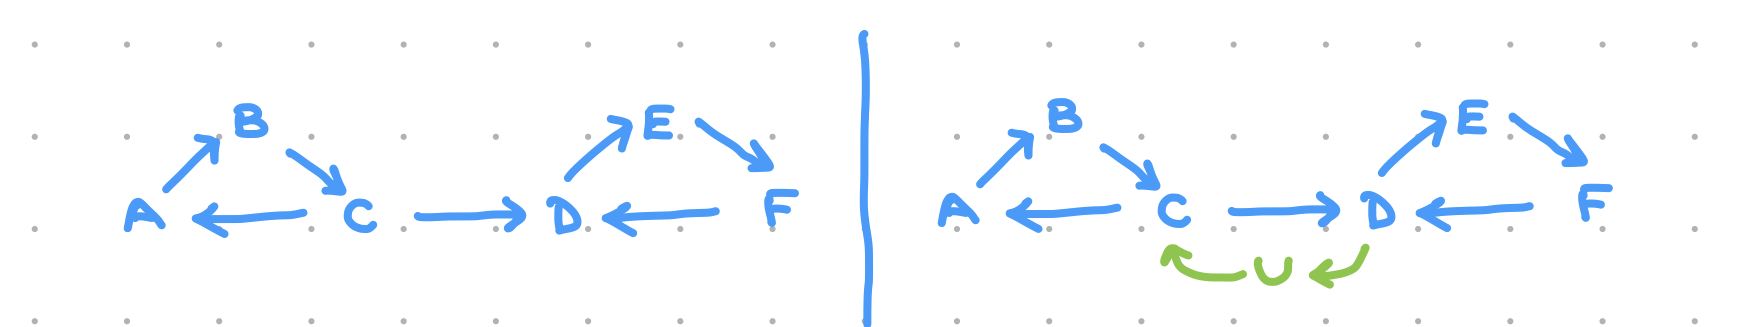
\includegraphics[width=0.9\textwidth]{src/CSE101 hw2 q3.png}


\item Give a characterization (an if and only if condition) of the minimum number of edges we must add,
in terms of the strongly connected components of $G$.

\-\ \newline 
The minimum number of edges \(E_m\) is given by
\[
E_m = S + K
\]

where K is the number of sink SCCs, and S is the number of source SCCs.
\-\ \newline

\item Describe how to use an algorithm from class to compute this number.

\begin {enumerate}
\item Run the Tarjan-Koseraju algorithm to find all SCCs within the graph. 
\item Check whether each SCC is a sink in G by running a DFS algorithm on it. If a node outside the SCC is reachable, it is not a sink. If the only nodes that are reachable are those in the SCC, it is a sink.
\item Repeat items \(i, ii\) for the reverse graph to find its sinks, and thus the regular graph's sources. 

\end {enumerate}

\-\ \newline
\item How long would this algorithm take to do this?  Explain.  

\-\ \newline

The algorithm runs in \(O( |V| (|V| + |E|) )\)

\begin {enumerate}
\item The two Tarjan-Koseraju algorithms run in \(O(|V + |E|)\) time.
\item Each DFS call runs in \(O(|V| + |E|)\), and is run for every vertex at most twice. 
\item Thus the total algorithm takes \(O(|V|(|V| + |E|))\)
\end {enumerate}

\end{enumerate}

%--------------------- Question 4 ---------------------
\newpage
\item

\end{enumerate}
\end{document}

